\documentclass{article}

\usepackage[
backend=biber,
style=numeric,
sorting=ynt
]{biblatex}
\addbibresource{refs.bib}

\usepackage{soul}
\usepackage{ifthen}
\usepackage[makeroom]{cancel}
\usepackage{amsthm}
\usepackage{amsmath}
\usepackage{amssymb}
\usepackage{mathtools}
\usepackage{needspace}
\usepackage{etoolbox}
\usepackage{listofitems}
\usepackage{xstring}
\usepackage{graphicx} % Required for inserting images
\usepackage{tikz}
\usetikzlibrary{patterns}
\usetikzlibrary{external}

\newtheorem{theorem}{Theorem}
\newtheorem{definition}{Definition}
\newtheorem{lemma}{Lemma}
\newtheorem{example}{Example}

\preto{\lemma}{\needspace{4cm}}
\preto{\section}{\needspace{5cm}}
\preto{\subsection}{\needspace{3cm}}
\preto{\example}{\needspace{3cm}}

\title{Heart of the Four Color Theorem}
\author{Timothy van der Valk}
\date{November 2024 - January 2025}

\newcommand{\I}{\text{I}}
\newcommand{\II}{\text{II}}
\newcommand{\compat}{\implies}
\newcommand{\ncompat}[1]{\stackrel{#1}{\compat}}
\newcommand{\digitToNum}[1]{\the\numexpr#1\relax}
\newcommand{\scheme}[2]{
    \readlist*\mylist{#2}
     \tikz[baseline]{ 
        \foreach \x [count=\i] in {#1} {
            \coordinate (\i) at (0.3*\i, 0.225); \node[text height=0mm] at (0.3*\i,0) {$\x$};
        } 
        \foreachitem \z \in \mylist {
            \StrChar{\z}{1}[\left]
            \StrChar{\z}{2}[\right]
            \StrChar{\z}{3}[\color]
            \StrChar{\z}{4}[\cross]
            \path (\left) edge[bend left=45] node[above, yshift=-2]{\small 
            \ifthenelse{\equal{\cross}{-}}{$\cancel{\color}$}{$\color$}
            } (\right);
        }
    }
} 

\begin{document}

\maketitle

A new proof of the four-color theorem has been given by Thomas et al \cite{thomas} in 1995 as a response to the Appel and Haken proof from 1976. Both proofs of the four-color theorem depend on three smaller theorems and a set of configurations that together contradict the existence of a minimal counterexample. The difference is that the new proof has a set of 633 configurations compared to 1476 members of the old one.

This document elaborates on the key concepts and results of reducibility underlying the four color theorem. The theory is built up from an intuitive and chronological point of view. Every definition is strongly motivated before being introduced. Ring reducibility results of Birkhoff have been rewritten using solid definitions and new notation and figures are included for most intuitive explanations. In addition, several examples of the types of reducibility are given. The C-reducibility of the Birkhoff diamond is proven and its full reducibility structure is visualised.

\tableofcontents

\pagebreak
\section{Introduction}

The four-color theorem is proven by disproving the existence of minimal counterexamples. Let us begin by defining such a minimal counterexample.
\begin{definition}
A graph $G$ is a minimal counterexample to the four-color theorem if $G$ is not four-colorable but any graph $H$ of lower weight $|V(H)|+|E(H)|$ is.
\end{definition}

All minimal counterexamples we mention will be those of the four-color theorem.
The three theorems to the four-color theorem are then as follows. We leave further definitions to Sections \ref{sec:birkhoff} and \ref{sec:config}.

\begin{theorem}
Minimal counterexamples are Birkhoff graphs.
\end{theorem}

\begin{theorem}
Minimal counterexamples do not contain configurations.
\end{theorem}

\begin{theorem}
Birkhoff graphs contain a configuration.
\end{theorem}

Clearly these three results contradict each other. Minimal counterexamples are proven to have no configurations, but subsequently through Birkhoff graphs, do in fact have configurations. This is a contradiction. As a consequence, there can not exist any minimal counterexamples and the four-color theorem is true. 

Theorem 1 is proven by hand in Section \ref{sec:birkhoff}. Theorem 2 and 3 are explained in Section \ref{sec:config} but require a computer to verify all cases. Birkhoff graphs are also called "internally 6-connected triangulations" in literature, but we will use the former for readability.

\section{Birkhoff Reducibility}
\label{sec:birkhoff}

Before 1913, the only known reductions of maps we're the reductions to triangulations and the reduction of multiply-connected regions to fewer regions (holed regions). In 1913, Birkhoff \cite{birkhoff} proved a new reduction result for \textit{rings} that seperate two parts of a map. This result spurred new developments in the reduction of graphs that opened the path towards reducible configurations and finally the proof of Appel and Haken in 1976.

We will use the term \textit{map} to refer to a map of connected \textit{regions} that we wish to four-color. From such a map we can construct a \textit{planar graph} where each region represents a vertex. We will be working with graphs in all our proofs, but might sometimes mention maps for intuition. We denote by $|G|$ the number of vertices in the graph $G$.

Let us begin by defining a ring of a graph.

\begin{definition}
    A ring of $n$ vertices $R_n$ in a graph $G$ is an induced cycle of $G$ that encloses at least one vertex.
\end{definition}

The key property of rings is that they seperate the full graph $G$ in three parts $M_1$, $R$ and $M_2$. That is, $G$ is of the form $G = M_1 + R + M_2$. The notation $A + B$ indicates a \textbf{direct} connection between the subgraphs $A$ and $B$. Since the ring seperates $M_1$ and $M_2$, they are not directly connected together.

\begin{figure}[!ht]
    \centering
        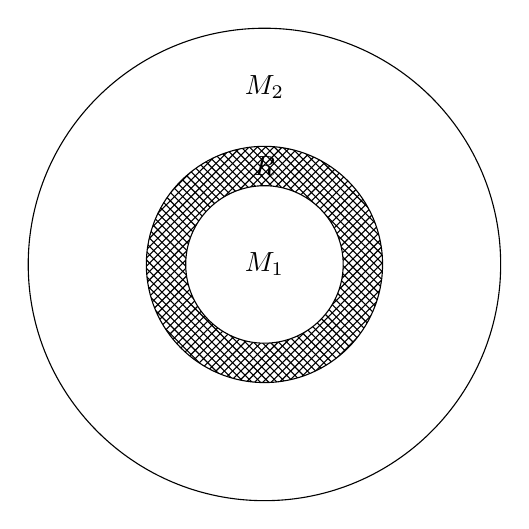
\begin{tikzpicture}
        \draw[fill=white] (0,0) circle (3cm);
        \draw[fill opacity=0.4, pattern=crosshatch] (0,0) circle (1.5cm);
        \draw[fill=white] (0,0) circle (1cm);
        \node at (0, 1.25) {$R$};
        \node at (0, 2.25) {$M_2$};
        \node at (0, 0) {$M_1$};
    \end{tikzpicture}
    \caption{The graph $G = M_1 + R + M_2$.}
\end{figure}

To reduce a ring like this, we may try to color $M_1+R$ and $M_2+R$ individually such that the colors on $R$ agree. Then we can combine both colorings together to form a coloring of the full graph $G$. This is the key idea of Birkhoff reducibility.

However, we do not know if such a common coloring of $M_1+R$ and $M_2+R$ always exists. Birkhoff's paper concerned itself with the conditions under which this, or a weaker result, is possible.

\subsection{Kempe Chains and Ring Schemes}

To make our coloring proofs easier, we need some definitions and notation to rewrite one coloring to another more easily. We will begin by defining chains of alternating colors connected to a vertex $v$.

\begin{definition}
    Given two colors $a,b$ and a coloring of a graph $G$. The $ab$-chain of a vertex $v \in G$ consists of all vertices colored $a,b$ that are connected to $v$ through other vertices colored $a,b$.
\end{definition}

Given a coloring of $M+R$. Consider the $ab$-chains of two vertices $v_1$ and $v_2$ on the ring $R$. If these chains are connected, then we may flip the colors in both $ab$-chains together to obtain a single new coloring. If these chains are not connected, then we may flip each $ab$-chain individually to obtain three new colorings ($\circ \bullet, \bullet \circ$ and $ \bullet \bullet$) instead.

Therefore, by using the concept of chains we can rewrite one coloring to another given knowledge of the chains that are present. To know which chains are present on a ring $R$, we also introduce the concept of a \textbf{ring scheme}.

\begin{definition}
    A ring scheme consists of the colors of a ring $R_n$ where two colors of the scheme are connected by a line if the corresponding vertices are connected by a chain. The colors in the chain are indicated above the line.
\end{definition}

For example, \scheme{a,b,a,b}{13c} indicates that the ring is colored $abab$ with a chain connecting $v_1$ and $v_3$.

\begin{figure}[!ht]
    \centering
    
    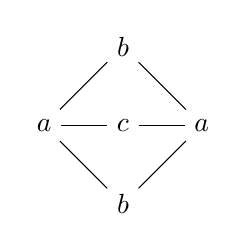
\begin{tikzpicture}
        % Define the nodes
        \node (v1) at (-1, 0) {$a$};
        \node (v2) at (0, 1) {$b$};
        \node (v3) at (1, 0) {$a$};
        \node (v4) at (0, -1) {$b$};
        \node (c) at (0, 0) {$c$};

        % Draw the edges
        \draw (v1) -- (v2) -- (v3) -- (v4) -- (v1);
        \draw (v1) -- (c) -- (v3);
    \end{tikzpicture}
    \caption{A graph that is colored $abab$ and has an $ac$-chain.}
\end{figure}

Now given the scheme \scheme{a,b,a,b}{13c}, we know certainly that there can not exist a $bd$-chain connecting $v_2$ and $v_4$ on the same side as the $ac$-chain. See the above graph, for example. Thus we can flip $v_2$ safely to obtain a new coloring $adab$. In such a case we write $\scheme{a,b,a,b}{13c} \cong \scheme{a,d,a,b}{13c}$. In addition, we write $abab \cong \scheme{a,b,a,b}{13d}$ to state that the coloring $abab$ has the specified ring scheme.

In general, if there is a chain connecting two vertices on the ring, then there can not exist a chain in complementary colors connecting two vertices seperated by that chain on the same ring.

\subsection{Ring Reducibility Numbers $\phi(n)$}

As we will prove in the next two sections, we can reduce the coloring of a graph containing the rings $R_4$ and $R_5$ as follows.

\begin{figure}[!ht]
    \centering
    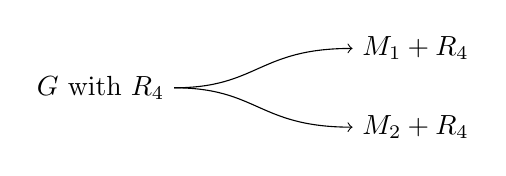
\begin{tikzpicture}
        \node (r4) at (-5, 0) {$G$ with $R_4$};
        \node (r4a) at (-1, 0.5) {$M_1+R_4$};
        \node (r4b) at (-1, -0.5) {$M_2+R_4$};
        \draw[->] (r4) .. controls +(2, 0) and (-3, 0.5) ..(r4a);
        \draw[->] (r4) .. controls +(2, 0) and (-3, -0.5) ..(r4b);
    \end{tikzpicture}
    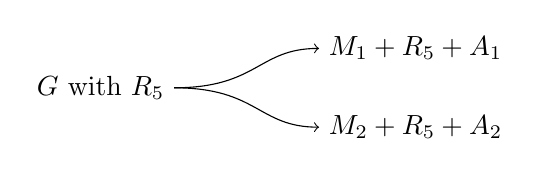
\begin{tikzpicture}
        \node (r4) at (-5, 0) {$G$ with $R_5$};
        \node (r4a) at (-1, 0.5) {$M_1+R_5+A_1$};
        \node (r4b) at (-1, -0.5) {$M_2+R_5+A_2$};
        \draw[->] (r4) .. controls +(2, 0) and (-3, 0.5) ..(r4a);
        \draw[->] (r4) .. controls +(2, 0) and (-3, -0.5) ..(r4b);
    \end{tikzpicture}
    \caption{The two key results of ring reducibility by Birkhoff. Rings of size 5 can only be reduced with auxiliary vertices $|A_1|=1$ and $|A_2| \leq 1$.}
\end{figure}

We have that rings of size 4 can be reduced exactly as we sought. However, for rings of size 5, at least one of the reduced graphs requires an auxiliary vertex. This is a slightly weaker result. In fact, the larger the ring size, the more auxiliary vertices will be required.

Birkhoff identified this as the generalization of ring reducibility and gave it a definition. 

\begin{definition}
    Let $\phi(n) = k$ where $k$ is the lowest integer such that all graphs $M_1+R_n+A_1$ and $M_2+R_n+A_2$ have a common ring coloring on $R_n$ for some $A_1$ and $A_2$ with $|A_1|=k$ and $|A_2|\leq k$ that are connected to all vertices of $R_n$.
\end{definition} 

We will be able to reduce graphs with rings of size $n$ to two \textbf{smaller}  graphs as long as $M_1$ and $M_2$ both contain more than $\phi(n)$ vertices. Otherwise, we would be reducing to a graph $|M+R_n+A| = |G|$, which is useless.

\subsection{Proof that $\phi(4)=0$}

We are now ready to prove that rings of size 4 are reducible without auxiliary regions ($k=0$). Let the ring colorings of $M_1+R_4$ be given by I, and the ring colorings of $M_2+R_4$ by II. 

Since we can reduce cycles of size greater than three to triangles, we can color two vertices on the ring $R_4$ the same. We can merge either $v_1$ and $v_3$, or $v_2$ and $v_4$. This results in colorings $a{*}a{*}$ and ${*}a{*}a$ where the $*$ are yet to be decided.

If the ring requires only two colors, then the only coloring we get is of the form $abab$. If the ring requires three colors, we get either $abac$ or $baca$ (up to permutation). Therefore we have two sets of choices for I and II.

\begin{equation*}
    abab, \quad\quad abac+baca
\end{equation*}

If I and II have the same type of coloring, we are done. Therefore, suppose that we have $\text{I}(abab)$  and $\text{II}(abac+baca)$. We will show that $abab$ can be rewritten to a coloring for II by branching on the existence of chains.

Suppose that there is an $ad$-chain connecting $v_1$ and $v_3$ in $\text{I}(abab)$. Then we have
\begin{equation*}
    \text{I}(abab) \cong \scheme{a,b,a,b}{13d}  \cong \text{II}(abac)
\end{equation*}

If there is no such chain, we must have a $bc$-chain connecting $v_2$ and $v_4$ such that 
\begin{equation*}
    \text{I}(abab) \cong \scheme{a,b,a,b}{24c} \cong \text{II}(baca)
\end{equation*}

In either case we get that $|\text{I} \cap \text{II}| > 0$, i.e there is a common ring coloring of $M_1+R_4$ and $M_2+R_4$. Hence $\phi(4) = 0$ since no auxiliary vertices we're used.

\subsection{Proof that $\phi(5)\leq1$}

To prove that $\phi(5)=1$, we first show that we can always find a common coloring of $M_1+R_5+A_1$ and $M_2+R_5+A_2$ if $|A_1|=1$ and $|A_2|\leq 1$ such that $\phi(5) \leq 1$. Then we give a counterexample such that $\phi(5)\neq 0$.

Let us consider the ring colorings I of the graph $M_1 + R_5 + A_1$. We have a single auxiliary vertex in $A_1$ that is connected to all vertices of the ring $R_5$. Since we can use only four colors, the ring has three colors with the last being used on $A_1$. Therefore we have \textbf{one of} the colorings

\begin{equation*}
    \vec{\underline{c}}abab = \begin{cases}
        cabab, \\
        acbab, \\
        abcab, \\
        abacb, \\
        ababc
    \end{cases}
\end{equation*}

The shorthand $\vec{c}abab$ indicates that $c$ can change position freely. We can only assume to have one of these colorings in I. The underlined vertex is called the \textbf{marked vertex}. This is the uniquely colored vertex in a three-coloring. Two three-colorings are called \textbf{adjacent} if the marked vertices are adjacent. 

Now for the ring colorings II of the graph $M_2+R_5+A_2$ we may consider $|A_2|=0$ and $1$. We have the colorings for $|A_2|=1$ as above. For $|A_2|=0$, we will be left with $M_2+R_5$. Again, cycles of size greater than three may be reduced by merging any two opposite vertices. This results in \textbf{all of} the following colorings

\begin{equation*}
    \vec{\underline{c}}abab, \quad\quad
    +\vec{a}{*}\vec{a}{*}{*} = \begin{cases}
        a{*}a{*}{*}+ \\
        {*}a{*}a{*}+ \\
        {*}{*}a{*}a+ \\
        a{*}{*}a{*}+ \\
        {*}a{*}{*}a
    \end{cases}
\end{equation*}

Here the shorthand $+\vec{a}{*}\vec{a}{*}{*}$ to indicates that the we have \textbf{all} valid colorings where $a$ can change position freely. The starred colors \textbf{depend} on the positions of $a$. Each coloring requires either three or four colors.

Now we can begin to show that there is a common ring coloring in I and II. We will do this by proving the following two lemmas.

\begin{lemma}
    \label{r5lem1}
    If I and II have two non-adjacent colorings, then they either have adjacent colorings or a common coloring.
\end{lemma}

\begin{lemma}
    \label{r5lem2}
    If I and II have two adjacent colorings, then they have a common coloring.
\end{lemma}

Together these two lemmas imply that regardless of whether the two colorings $\vec{\underline{c}}abab$ in I and II are adjacent or non-adjacent, there will be a common coloring. If the marked vertices are the same, we can simply permute colors to obtain a common coloring.

\vspace{1em}
\emph{Proof of Lemma \ref{r5lem1}}

Assume we have two non-adjacent colorings $\text{I}(ab\underline{c}ab)$ and $\text{II}(\underline{c}abab)$. If a $bc$-chain connects $v_3$ and $v_4$ in $\text{I}(ab\underline{c}ab)$, then we obtain

\begin{equation*}
    \text{I}(ab\underline{c}ab) \cong \scheme{a,b,c,a,b}{35} \cong \text{I}(abcdb)
\end{equation*}

Let us now consider the coloring $\text{II}({*}b{*}{*}b)$. We must certainly use three colors, so we have at least $\text{II}({*}bcdb)$ with three options for the last color.

\begin{equation*}
    \text{II}({*}bcdb) \cong \begin{cases}
        \text{II}(abcdb) \cong& \text{I}(abcdb), \\
        \text{II}(cbc\underline{d}b) \quad \text{adjacent to} \quad& \text{I}(ab\underline{c}ab), \\
        \text{II}(db\underline{c}db) \cong& \text{I}(ab\underline{c}db)
    \end{cases}
\end{equation*}

In all three cases, we either have a common coloring or an adjacent coloring in I and II. If a $bc$-chain did not exist, then we have an $ad$-chain between $v_1$ and $v_4$ such that 

\begin{equation*}
    \text{I}(ab\underline{c}ab) \cong \scheme{a,b,c,a,b}{14d} \cong \text{I}(a\underline{c}bab)\quad \text{adjacent to}\quad \text{II}(\underline{c}abab).
\end{equation*}

An equivalent argument holds for all other pairs of non-adjacent colorings. Therefore we have either an adjacent coloring or a common coloring in I and II regardless of the colorings in I and II.

\vspace{1em}
\emph{Proof of Lemma \ref{r5lem2}}

Assume we have $\text{I}(a\underline{c}bab)$ and $\text{II}(\underline{c}abab)$. If a $bc$-chain connects $v_2$ and $v_4$ in $\text{I}(b\underline{c}aba)$, then we obtain

\begin{equation*}
    \text{I}(b\underline{c}aba) \cong \scheme{b,c,a,b,a}{24} \cong \text{I}(bcdba)
\end{equation*}

Now consider the coloring $\text{II}(b{*}{*}b{*})$. We again have three cases for this coloring starting from $\text{II}(bcdb{*})$.

\begin{equation*}
    \text{II}(bcdb{*}) \cong \begin{cases}
        \text{II}(bcdba) \cong& \text{I}(bcdba), \\
        \text{II}(bc\underline{d}bc) \\
        \text{II}(b\underline{c}dbd) \cong& \text{I}(a\underline{c}bab)
    \end{cases}
\end{equation*}

Now in case we obtain the coloring $\text{II}(bc\underline{d}bc)$, we have essentially shifted two steps right from $\text{II}(\underline{c}abab)$. If we repeat the same argument with $\text{II}(bc\underline{d}bc)$ and $\text{I}(a\underline{c}bab)$, we will obtain $\text{I}(aba\underline{c}b)$. Hence by repetition we get the colorings

\begin{equation*}
    \stackrel{\text{start}}{\text{I}(a\underline{c}bab)} \rightarrow 
    \text{I}(aba\underline{c}b) \rightarrow 
    \text{I}(\underline{c}abab) \cong \text{II}(\underline{c}abab)
\end{equation*}

The same repetition argument holds for all other pairs of adjacent colorings in I and II too. Therefore, if there adjacent colorings in I and II, then we obtain a common coloring of I and II.

Since we have proven both Lemma's, we conclude that the ring of five regions is reducible with $\phi(5) \leq 1$.

\subsection{Proof that $\phi(5) \neq 0$}

To prove that $\phi(5) \neq 0$, we must give an example of two  of graphs $M_1+R_5$ and $M_2+R_5$ such that there is no common ring coloring.


\section{D-Reducibility}
\label{sec:dreduce}

\subsection{Definitions}

The proof of the four-color theorem consists of proving that every graph has a certain subgraph that can be reduced to a smaller graph. So far, we have proven reducibility only for graphs containing the rings $R_4$ and $R_5$. The graphs that we we're left with we called Birkhoff graphs.

Since Birkhoff graphs already contain a lot of structure and information, our hopes are that every such Birkhoff graph contains \textbf{at least one subgraph of a finite set of reducible subgraphs}. We will call these subgraphs \textit{configurations}.

\begin{definition}
    A configuration is a triangulation where the outer vertices form a ring $R_n$ of size $n \geq 4$.
\end{definition}

An example of a configuration is the \textit{Birkhoff diamond} visible in Figure \ref{fig:diamond} of Section \ref{sec:diamond} which was proven to be reducible by Birkhoff \cite{birkhoff}.

We have seen the notion of one ring scheme \textit{implying} another by means of a flipping of color chains. Consider now a single coloring say $abab$ of $R_4$. By conditioning on the presence of an $ad$-chain, we obtain two implied colorings.

\begin{equation*}
    \scheme{a,b,a,b}{{13d}} \compat abac
    \quad\text{or}\quad
    \scheme{a,b,a,b}{13d-} \compat abcb.
\end{equation*}

We therefore know with certainty that $abab$ implies either $abac$ or $abcb$. In such a case we write $abab \compat \{ abac, abcb \}$.

\begin{definition}
    A ring coloring $x$ implies a set of ring colorings $\II$ if for some pair of colors $ab$, all possible $ab$-chain schemes on $x$ imply a coloring of $\II$. We write $x \compat \II$.
\end{definition}

We can extend this to a set of colorings $\I$ implying $\II$ if all colorings of $x \in \I$ imply $\II$.

\begin{definition}
    A set of ring colorings $\I$ implies another set of ring colorings $\II$ if every $x \in \I$ implies $\II$. We write $\I \compat \II$.
\end{definition}

If you think about these definitions for a while, you will realize that the proofs of ring reducibility in Section \ref{sec:birkhoff} are mostly about proving that one set of ring colorings implies another.

How can we utilize this concept of implied sets to define a notion of reducibility for configurations? Given a configuration $C$, let us start by defining the sets of possible ring colorings of $C$ and a ring $R_n$.

\begin{definition}
    Let $\Phi_0(C)$ be the set of all ring colorings of a configuration $C$. Let $\Phi(n)$ be the set of all ring colorings of $R_n$.
\end{definition}

Consider an arbitrary ring coloring $x \in \Phi(n)$. If $x \in \Phi_0(C)$, then clearly we may reduce this configuration. Now using the concept of implying sets, let $\Phi_1(C)$ be the largest set such that $\Phi_1(C) \implies \Phi_0(C)$. Then every coloring in $\Phi_1(C)$ can be turned into a coloring of $\Phi_0(C)$ regardless of the chains present. Thus if $x \in \Phi_1(C)$, we are again reducible.

We can continue constructing sets of higher-level implication $\Phi_n(C)$ and each of the colorings in these sets can be used to reduce our configuration. Note that these sets are increasing in size, containing the previous set as well. That is $\Phi_n(C) \subset \Phi_{n+1}(C)$. Since these sets can not grow bigger than the set of all ring colorings $\Phi(n)$, there exists a largest such set $\overline{\Phi}(C) = \Phi_k(C)$ for some $k > 0$.

Finally, our configuration is D-reducible if this maximal set $\overline{\Phi}(C)$ is the set of all possible ring colorings $\Phi(n)$. Since in this case every coloring can be converted into a coloring for $C$ with chain flips.  Let us now define this intuition properly. Starting with higher-order implication.

\begin{definition}
    A set of ring colorings I $n$-implies another set II written as $\I \ncompat{n} \II$ if for some sets $B_{i}$ with $0 < i < n$,

    \begin{equation*}
        I \compat B_{n-1} \compat  \ldots \compat B_{1} \compat \II.
    \end{equation*}
\end{definition}

Using this definition, we will define the $n$-implying sets of a configuration $C$.

\begin{definition}
    The $n$-implying set $\Phi_n(C)$ of a configuration $C$ is the largest set of ring colorings such that $\Phi_n(C) \ncompat{n} \Phi_0(C)$.
\end{definition}

Finally, we define the largest implying set simply as \textit{the} implying set.

\begin{definition}
    The implying set $\overline{\Phi}(C)$ of a configuration $C$ is the largest $n$-implying set $\Phi_n(C)$ for some $n$ of $C$.
\end{definition}

With all these definitions in place, we can define the notion of D-reducibility.

\begin{definition}
    A configuration $C$ of ring size $n$ is D-reducible if $\overline{\Phi}(C) = \Phi(n)$.
\end{definition}

\begin{figure}[!h]
    \centering
    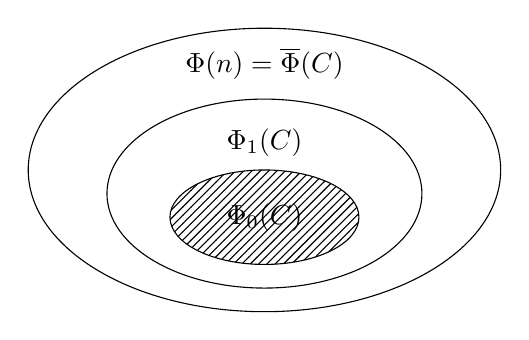
\begin{tikzpicture}[scale=1.0]
        \draw (0, 0) ellipse (3cm and 1.8cm);
        \draw (0, -0.3) ellipse (2cm and 1.2cm);
        \draw[fill opacity=0.4, pattern=north east lines] (0, -0.6) ellipse (1.2cm and 0.6cm);

        \node at (0.0, -0.6) { $\Phi_0(C)$ };
        \node at (0.0, 0.35) { $\Phi_1(C)$ };
        \node at (0, 1.35) { $\Phi(n) = \overline{\Phi}(C)$ };
    \end{tikzpicture}

    \caption{D-reducibility requires that all ring colorings can be converted to a valid ring coloring of $C$ in $\Phi_0(C)$.}
\end{figure}

Let us now view some simple examples of D-reducibility. A detailed example about the Birkhoff diamond can be found in Section \ref{sec:diamond}.

\subsection{Reducibility of the 4-star and 5-star}

For examples with and without D-reducibility, we look at the 4-star and 5-star respectively. They are pictured below.

\begin{figure}[!h]
    \centering
    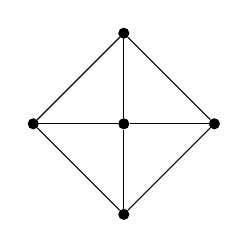
\begin{tikzpicture}[scale=1.15]
        \node[circle, fill, scale=0.015cm] (c) at (0, 0) {};
        \node[circle, fill, scale=0.015cm] (l1) at (1, 0) { };
        \node[circle, fill, scale=0.015cm] (l2) at (0, -1) { };
        \node[circle, fill, scale=0.015cm] (l3) at (-1, 0) {};
        \node[circle, fill, scale=0.015cm] (l4) at (0, 1) {};

        \draw (c) -- (l1);
        \draw (c) -- (l2);
        \draw (c) -- (l3);
        \draw (c) -- (l4);
        \draw (l1) -- (l2) -- (l3) -- (l4) -- (l1);

    \end{tikzpicture}
    \hspace{0.5cm}
    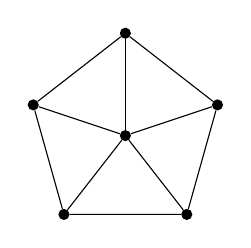
\begin{tikzpicture}[scale=1.3]
        \node[circle, fill, scale=0.015cm] (c) at (0, 0) {};
        \node[circle, fill, scale=0.015cm] (l1) at (0, 1) { };
        \node[circle, fill, scale=0.015cm] (l2) at (0.9, 0.30) { };
        \node[circle, fill, scale=0.015cm] (l3) at (0.6, -0.77) {};
        \node[circle, fill, scale=0.015cm] (l4) at (-0.6, -0.77) {};
        \node[circle, fill, scale=0.015cm] (l5) at (-0.9, 0.30) {};

        \draw (c) -- (l1);
        \draw (c) -- (l2);
        \draw (c) -- (l3);
        \draw (c) -- (l4);
        \draw (c) -- (l5);
        \draw (l1) -- (l2) -- (l3) -- (l4) -- (l5) -- (l1);
    \end{tikzpicture}
    \caption{The 4-star and the 5-star.}
\end{figure}

For the 4-star, we know that the only colorings it allows on the ring are those with three colors or less. Hence

\begin{equation}
    \Phi_0(\text{4-star}) = \{ abab, abac, baca \}.
\end{equation}

However, the set of all ring colorings of $R_4$ also includes the coloring $abcd$.

\begin{equation}
    \Phi(4) = \{ abab, abac, baca, abcd \}.
\end{equation}

Therefore, to prove D-reducibility, we must show that $abcd \in \Phi_n(\text{4-star})$ for some $n$-implying set. In this case we obtain that

\begin{equation}
    \scheme{a,b,c,d}{13a} \compat abcb \quad \text{or} \quad \scheme{a,b,c,d}{13a-} \compat abad.
\end{equation}

Both of these colorings are in $\Phi_0(\text{4-star})$ up to permutation. Therefore

\begin{equation*}
    \Phi_1(\text{4-star}) = \{ abcd \}.
\end{equation*}

Hence $\overline{\Phi}(\text{4-star}) = \Phi(4)$ and we can conclude that the 4-star is D-reducible.

However, the 5-star is unfortunately not D-reducible (this would also prove the four color theorem). The problem can quickly be seen from the fact that any chain on a 4-coloring like $abcad$ implies both a 3-coloring and 4-coloring.

\begin{equation*}
    \scheme{a,b,c,a,d}{35c} \compat abcbd \quad \text{or} \quad \scheme{a,b,c,a,d}{35c-} \compat abcbd.
\end{equation*}

The actual proof involves evaluating many cases, which can be done with a computer.

Next we treat C-reducibility that serves as the final form of reducibility required for the four-color theorem.
\section{C-Reducibility}
\label{sec:creduce}

The original proof of the four color theorem used an unavoidable set of C or D reducible configurations. C-reducibility can be thought of as a stronger but more complicated form of D-reducibility. In 2009, John P. Steinberger gave an unavoidable set of D-reducible configurations. With this, C-reducibility is no longer required to prove the four color theorem. However, the concept of C-reducibility is still insightful. Therefore we explain it here.

\subsection{Definitions}

Recall that D-reducibility required that all possible ring colorings $\Phi(n)$ are in the implying set $\overline{\Phi}(C)$. If a configuration is not D-reducible, then there must be ring colorings in $\Phi(n)$ that are not in $\overline{\Phi}(C)$. These colorings can not be converted to coloring of $C$ by flipping Kempe-chains. It is these colorings that we want to avoid with C-reducibility. By replacing $C$ with a reducer $(S,\sigma)$ consisting of a smaller graph $S$ and a ring contraction $\sigma$ we can avoid these colorings. For this to happen, the un-contracted ring colorings of $(S,\sigma)$ denoted by $\Phi(S, \sigma)$ must be in $\overline{\Phi}(C)$.

\begin{figure}[!h]
    \centering
    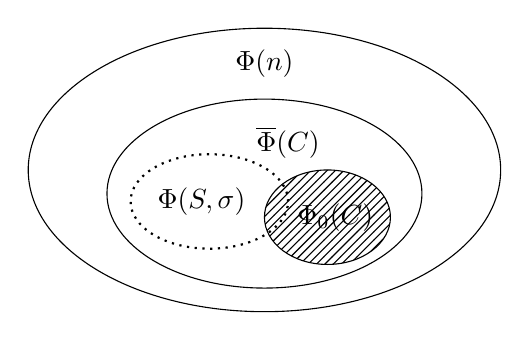
\begin{tikzpicture}[scale=1.0]
        \draw (0, 0) ellipse (3cm and 1.8cm);
        \draw (0, -0.3) ellipse (2cm and 1.2cm);
        \draw[fill opacity=0.4, pattern=north east lines] (0.8, -0.6) ellipse (0.8cm and 0.6cm);
        \draw[dotted, thick] (-0.7, -0.4) ellipse (1.0cm and 0.6cm);

        \node at (0.9, -0.6) { $\Phi_0(C)$ };
        \node at (0.3, 0.35) { $\overline{\Phi}(C)$ };
        \node at (0, 1.35) { $\Phi(n)$ };
        \node at (-0.8, -0.4) { $\Phi(S, \sigma)$ };
    \end{tikzpicture}

    \caption{C-reducibility requires that for some choice of a reducer $(S,\sigma)$, the colorings $\Phi(S, \sigma)$ can be converted to valid ring colorings of $C$ in $\Phi_0(C)$.}
    \label{fig:cred}
\end{figure}

Therefore, C-reducibility can be seen as an extension of D-reducibility with the reducer $(S, \sigma)$ acting as a "filter" of ring colorings. This way we can ignore those ring colorings that are not in $\overline{\Phi}(C)$. As can be seen in Figure \ref{fig:cred}, there are still colorings for the ring that are not in $\overline{\Phi}(C)$. However, we avoid them using the colorings of the reducer $\Phi(S, \sigma)$.

Let us start with the definition of a ring contraction.

\begin{definition}
    A ring contraction $\sigma(v)$ is a map from the vertices of a ring $R$ to the contracted ring $\sigma \circ R$. We require
    
    \begin{itemize}
        \item The contracted ring $\sigma \circ R$ is a valid planar graph.
        \item Neighboring ring vertices $v_i$ and $v_{i+1}$ are not contracted.
    \end{itemize}
\end{definition}

Ring contractions allows the reducer to shrink the number of boundary vertices. This simplifies the coloring problem for the reducer. Without a ring contraction, our reducer would still have the same ring as our configuration $C$, making it equally difficult to work with. Why do we not simply delete vertices from the ring of $C$? The contraction defines a map that allows us to convert boundary colorings of $(S,\sigma)$ to ring colorings of $C$ simply by un-contracting. 

\begin{figure}[!h]
    \centering
    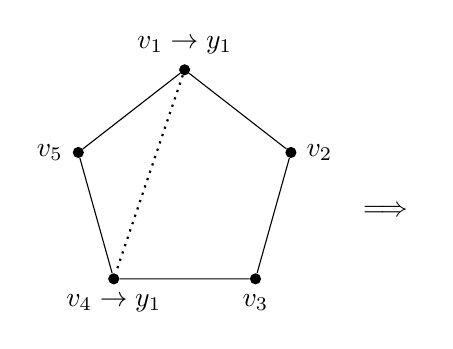
\begin{tikzpicture}[scale=1.5]
        \node[circle, fill, scale=0.015cm, label=above:{$v_1 \rightarrow y_1$}] (l1) at (0, 1) { };
        \node[circle, fill, scale=0.015cm, label=right:{$v_2$}] (l2) at (0.9, 0.30) { };
        \node[circle, fill, scale=0.015cm, label=below:{$v_3$}] (l3) at (0.6, -0.77) {};
        \node[circle, fill, scale=0.015cm, label=below:{$v_4 \rightarrow y_1$}] (l4) at (-0.6, -0.77) {};
        \node[circle, fill, scale=0.015cm, label=left:{$v_5$}] (l5) at (-0.9, 0.30) {};
        \draw (l1) -- (l2) -- (l3) -- (l4) -- (l5) -- (l1);
        \draw[dotted, thick] (l1) -- (l4);
        \node at (1.7, -0.2) { $\implies$ };
    \end{tikzpicture}
    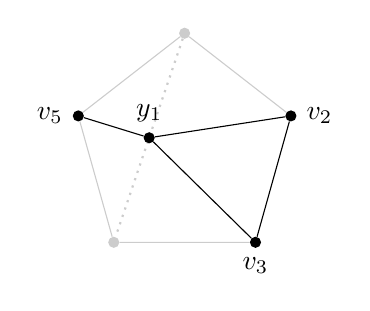
\begin{tikzpicture}[scale=1.5]
        \node[circle, fill, opacity=0.2, scale=0.015cm] (l1) at (0, 1) {};
        \node[circle, fill, opacity=0.2, scale=0.015cm] (l4) at (-0.6, -0.77) {};
        \node[circle, fill, scale=0.015cm, label=above:{$y_1$}] (y1) at (-0.3, 0.115) {};

        \node[circle, fill, scale=0.015cm, label=right:{$v_2$}] (l2) at (0.9, 0.30) { };
        \node[circle, fill, scale=0.015cm, label=below:{$v_3$}] (l3) at (0.6, -0.77) {};
        \node[circle, fill, scale=0.015cm, label=left:{$v_5$}] (l5) at (-0.9, 0.30) {};

        \draw (l5) -- (y1) -- (l2) -- (l3) -- (y1);
        \draw[dotted, thick, opacity=0.2] (l1) -- (l4);
        \draw[opacity=0.2] (l5) -- (l1) -- (l2);
        \draw[opacity=0.2] (l3) -- (l4) -- (l5);
    \end{tikzpicture}
    \caption{A contraction on $R_5$. The two vertices $v_1$ and $v_4$ are mapped to the same vertex $y_1$, and hence get contracted together. }
    \label{fig:contract}
\end{figure}

Figure \ref{fig:contract} shows the contraction process on $R_5$. Intuitively, you should think of a contraction as the merging of pairs of vertices to a single point. However, mathematically, it is easier to work with a mapping function $\sigma$ instead. Suppose we are given a coloring $x(v)$ of a contracted ring $\sigma \circ R$. Then the composition $x \circ \sigma(v)$ is a valid coloring for $R$. This is shown in Figure \ref{fig:contractcolor}

\begin{figure}[!h]
    \centering
    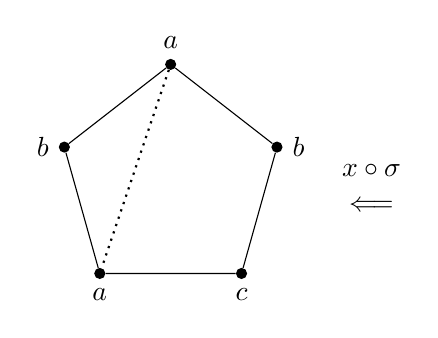
\begin{tikzpicture}[scale=1.5]
        \node[circle, fill, scale=0.015cm, label=above:{$a$}] (l1) at (0, 1) { };
        \node[circle, fill, scale=0.015cm, label=right:{$b$}] (l2) at (0.9, 0.30) { };
        \node[circle, fill, scale=0.015cm, label=below:{$c$}] (l3) at (0.6, -0.77) {};
        \node[circle, fill, scale=0.015cm, label=below:{$a$}] (l4) at (-0.6, -0.77) {};
        \node[circle, fill, scale=0.015cm, label=left:{$b$}] (l5) at (-0.9, 0.30) {};
        \draw (l1) -- (l2) -- (l3) -- (l4) -- (l5) -- (l1);
        \draw[dotted, thick] (l1) -- (l4);
        
        \node at (1.7, 0.1) { $x \circ \sigma$ };
        \node at (1.7, -0.2) { $\Longleftarrow$ };
    \end{tikzpicture}
    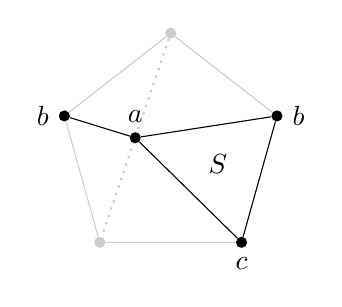
\begin{tikzpicture}[scale=1.5]
        \node[circle, fill, opacity=0.2, scale=0.015cm] (l1) at (0, 1) {};
        \node[circle, fill, opacity=0.2, scale=0.015cm] (l4) at (-0.6, -0.77) {};
        \node[circle, fill, scale=0.015cm, label=above:{$a$}] (y1) at (-0.3, 0.115) {};

        \node[circle, fill, scale=0.015cm, label=right:{$b$}] (l2) at (0.9, 0.30) { };
        \node[circle, fill, scale=0.015cm, label=below:{$c$}] (l3) at (0.6, -0.77) {};
        \node[circle, fill, scale=0.015cm, label=left:{$b$}] (l5) at (-0.9, 0.30) {};

        \draw (l5) -- (y1) -- (l2) -- (l3) -- (y1);
        \draw[dotted, thick, opacity=0.2] (l1) -- (l4);
        \draw[opacity=0.2] (l5) -- (l1) -- (l2);
        \draw[opacity=0.2] (l3) -- (l4) -- (l5);

        \node at (0.4, -0.11) { $S$ };
    \end{tikzpicture}
    \caption{ The coloring $x(v)$ of a contracted ring $\sigma \circ R$ can be converted to a coloring for the original ring $R$ using $x \circ \sigma(v)$. }
    \label{fig:contractcolor}
\end{figure}

By introducing ring contractions, we have already covered the most significant part of a reducer. The last part is the extra graph $S$ that defines the interior of our contracted ring. This extra graph $S$ is similar to the auxiliary graph $A$ that we used during the 1-reducibility proof of $R_5$. The boundary vertices of $S$ must be the same as the contracted ring $\sigma \circ R$. Now we have all the parts needed to define a reducer.

\begin{definition}
    A reducer of a configuration $C$ is a pair $(S, \sigma)$  consisting of a ring contraction $\sigma$ and a graph $S$ on less vertices than $C$ that has a boundary equal to the contracted ring $\sigma \circ R$.
\end{definition}

Of course, every reducer will reduce the size of a configuration $C$. However, for actual reducibility, we can not simply take any reducer. Our reducer $(S, \sigma)$ must satisfy the filtering property mentioned at the beginning of this section. That is, its ring colorings $\Phi(S, \sigma)$ must be contained in $\overline{\Phi}(C)$. Let us define this set.

\begin{definition}
    Let $(S, \sigma)$ be a reducer. The set of un-contracted ring colorings $\Phi(S, \sigma)$ consists of all the colorings $x \circ \sigma$ with $x(v)$ a boundary coloring of $S$.
\end{definition}

Following this definition, C-reducibility is a simple concept.

\begin{definition}
    A configuration $C$ is C-reducible if $\Phi(S,\sigma) \subset \overline{\Phi}(C)$ for some reducer $(S,\sigma)$.
\end{definition}

Now suppose we have a graph $G$ where $C$ is an embedded C-reducible configuration with reducer $(S,\sigma)$. Suppose that two non-neighboring ring vertices of $C$ are connected by an edge in $G$. If we would contract these vertices together, then we would create a loop on the boundary of $S$. We can not color vertices with loops without breaking the rules of a coloring. Therefore, we must take care to avoid such loops.

Since this issue is specific to the way the configuration $C$ is embedded in the graph $G$, we will give a name to the type of embedding that we are after.

\begin{definition}
    A configuration $C$ is $\sigma$-properly embedded in $G$ if two ring vertices of $C$ that are connected by an non-ring edge in $G$ are not contracted by $\sigma(v)$.
\end{definition}

\begin{definition}
    The C-reducible configuration $C$ has a safe reducer  $(S,\sigma)$ if it only occurs $\sigma$-properly embedded in a Birkhoff graph.
\end{definition}

Before we can use C-reducible configurations to reduce counterexamples, we must first prove the existence of a safe reducer. This was a major source of complications in the original proof of the four color theorem by Appel and Haken. This is a strong condition on the structure of a reducer. We will see examples of safe and unsafe reducers in the next section.

\subsection{C-Reducibility of the Birkhoff diamond}
\label{sec:diamond}

Although we have already shown that the Birkhoff diamond is D-reducible, we will use it as a slightly more interesting example of C-reducibility. A reducer for the Birkhoff diamond we have picture below.

\begin{figure}[!h]
    \centering
    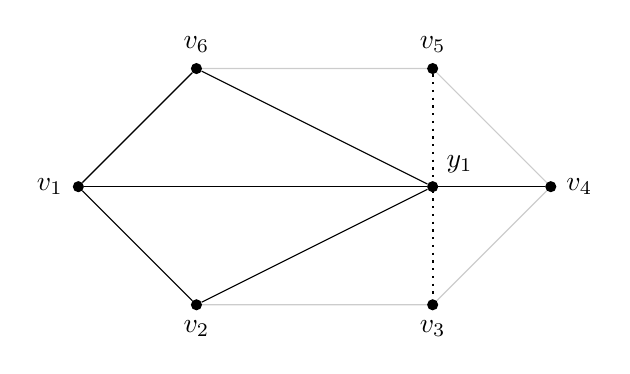
\begin{tikzpicture}[scale=1.5]
        \node[circle, fill, scale=0.015cm, label=left:$v_1$] (l1) at (-2, 0) { };
        \node[circle, fill, scale=0.015cm, label=above:$v_6$] (l2) at (-1, 1) { };
        \node[circle, fill, scale=0.015cm, label=below:$v_2$] (l4) at (-1, -1) {};

        \node[circle, fill, scale=0.015cm,label=right:$v_4$] (r1) at (2, 0) {};
        \node[circle, fill, scale=0.015cm,label=above:$v_5$] (r2) at (1, 1) {};
        \node[circle, fill, scale=0.015cm,label=below:$v_3$] (r4) at (1, -1) {};

        \node[circle, fill, scale=0.015cm,label=above right:$y_1$] (y1) at (1, 0) {};

        \draw[opacity=0.2] (l1) -- (l2) -- (r2) -- (r1) -- (r4) -- (l4) -- (l1);
        \draw[dotted, thick] (r2) -- (r4);
        \draw (l1) -- (l2) -- (y1) -- (l4) -- (l1);
        \draw (l1) -- (y1) -- (r1);
    \end{tikzpicture}
    \caption{A reducer for the Birkhoff diamond (in bold) with a single contraction on $v_4$ and $v_2$, and a single edge added by $S$. }.
    \label{fig:diamondreducer}
\end{figure}

Let us now prove the C-reducibility of the Birkhoff diamond with this reducer. First, we determine the set of colorings that the reducer creates for the original ring $R_6$.

\begin{equation}
    \Phi(S, \sigma) = \left\{ \begin{matrix}
        ababcd, & abcbdc, & abcbcd, \\ abcbac, & abcbad, & \underline{ababac}
    \end{matrix}\right\}
\end{equation}

By looking at Table \
\section{The Birkhoff Diamond}
\label{sec:diamond}

\begin{figure}[!h]
    \centering
    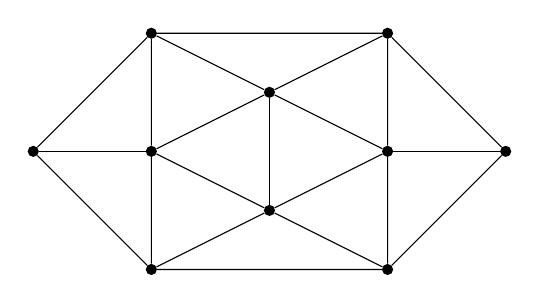
\begin{tikzpicture}[scale=1.5]
        \node[circle, fill, scale=0.015cm] (l1) at (-2, 0) { };
        \node[circle, fill, scale=0.015cm] (l2) at (-1, 1) { };
        \node[circle, fill, scale=0.015cm] (l3) at (-1, 0) {};
        \node[circle, fill, scale=0.015cm] (l4) at (-1, -1) {};

        \node[circle, fill, scale=0.015cm] (r1) at (2, 0) {};
        \node[circle, fill, scale=0.015cm] (r2) at (1, 1) {};
        \node[circle, fill, scale=0.015cm] (r3) at (1, 0) {};
        \node[circle, fill, scale=0.015cm] (r4) at (1, -1) {};

        \node[circle, fill, scale=0.015cm] (c1) at (0, 0.5) {};
        \node[circle, fill, scale=0.015cm] (c2) at (0, -0.5) {};

        \draw (l1) -- (l2) -- (r2) -- (r1) -- (r4) -- (l4) -- (l1);
        \draw (l1) -- (l3);
        \draw (l2) -- (l3) -- (l4);
        \draw (l2) -- (c1) -- (l3) -- (c2) -- (l4);
        \draw (c1) -- (c2);
        \draw (r2) -- (c1) -- (r3) -- (c2) -- (r4);
        \draw (r2) -- (r3) -- (r4);
        \draw (r1) -- (r3);
    \end{tikzpicture}
    \caption{The Birkhoff diamond with ring size 6}.
    \label{fig:diamond}
\end{figure}

\pagebreak
\printbibliography

\end{document}
